% Compile with:
% latexmk -pdf -pvc -interaction=nonstopmode
%\documentclass[aspectratio=169,draft]{beamer}
\documentclass[aspectratio=169]{beamer}
\usetheme{UniBern}

\title{Automated segmentation and description of the internal morphology of human permanent teeth}
\author{David Haberthür}
\date{October 12, 2021 | \href{https://www.bruker.com/en/news-and-events/events/microCT_user_meeting_2021.html}{Bruker microCT User Meeting 2021}}

%\includeonlyframes{current}
%then....
%\begin{frame}[label=current]
%\end{frame}

\usepackage[detect-all=true,
	range-phrase=--,
	range-units=single,
	binary-units=true,
	per-mode=symbol,
	per-symbol=/]{siunitx}
\usepackage{xspace}
\usepackage{gitinfo2}
\usepackage[backend=biber,
	style=numeric,
	url=false,
	maxnames=1,
	sorting=none,
	]{biblatex}
%\addbibresource{~/P/Documents/library.bib}
\addbibresource{~/Desktop//library.bib}
%\addbibresource{../../Documents/library.bib}
\usepackage{ccicons}
\usepackage{animate}
\usepackage{tikz}
	\usetikzlibrary{spy}
	\tikzset{shadowed/.style={preaction={transform canvas={shift={(1pt,-1pt)}},draw=ubRed}}}
\usepackage{shadowtext} % for the shadowed scalebar
	\shadowoffset{1pt}
	\shadowcolor{ubRed}
\usepackage[absolute,overlay]{textpos} % for the \source* command
\usepackage{fontawesome5}
\usepackage{listings}
	\lstset{frame=single,
	basicstyle=\tiny\ttfamily
	}
\usepackage{booktabs}
\usepackage{multirow}
\usepackage{colortbl}
\usepackage{adjustbox}
\usepackage{microtype}

% Some often used abbreviations/commands
\newcommand{\everyframe}{2} % use only every nth frame for the animations
\newcommand{\imwidth}{\linewidth}% set global image width
\newcommand{\imheight}{0.8\paperheight}% set global image height
\newlength\imagewidth% needed for scalebars
\newlength\imagescale% needed for scalebars
\newcommand{\uct}{\si{\micro}CT\xspace}% make our life easier
\newcommand{\eg}{e.\,g.\xspace}%
\newcommand{\ie}{i.\,e.\xspace}%

% Define complementary colors to ubRed
\definecolor{ubRedComplementary1}{HTML}{00a1e6}
\definecolor{ubRedComplementary2}{HTML}{00e645}

% Acknowledge images just below them
% Based on https://tex.stackexchange.com/a/282637/828
\newcommand{\source}[2]{%
	% Print out (short) link under image, with small text
	\raisebox{-1.618ex}{%
		\makebox[0pt][r]{%
			\scriptsize\href{http://#1}{#1} #2%
			}%
		}%
	}%
\newcommand{\sourcecite}[2]{%
	% Cite (an image from) a reference
	\raisebox{-1.618ex}{%
		\makebox[0pt][r]{%
			\scriptsize From \cite{#1}, #2%
			}%
		}%
	}%
\newcommand{\sourcelink}[3]{%
	% Make the source command an \href{link}{text}
	\raisebox{-1.618ex}{%
		\makebox[0pt][r]{%
			\scriptsize\href{http://#1}{#2}, #3%
			}%
		}%
	}%

% Define us a custom footer *with* progress bar, based on https://tex.stackexchange.com/a/59749/828
\makeatletter
\def\progressbar@progressbar{} % the progress bar
\newcount\progressbar@tmpcounta% auxiliary counter
\newcount\progressbar@tmpcountb% auxiliary counter
\newdimen\progressbar@pbht %progressbar height
\newdimen\progressbar@pbwd %progressbar width
\newdimen\progressbar@rcircle % radius for the circle
\newdimen\progressbar@tmpdim % auxiliary dimension
\progressbar@pbwd=0.85\linewidth
\progressbar@rcircle=1.5pt
\def\progressbar@progressbar{%
	\progressbar@tmpcounta=\insertframenumber
	\progressbar@tmpcountb=\inserttotalframenumber
	\progressbar@tmpdim=\progressbar@pbwd
	\multiply\progressbar@tmpdim by \progressbar@tmpcounta
	\divide\progressbar@tmpdim by \progressbar@tmpcountb
	\par%
	\begin{tikzpicture}%
		\draw[ubGrey] (0,0) -- ++ (\progressbar@pbwd,0);
		\draw[draw=ubRed,fill=ubGrey] (\the\dimexpr\progressbar@tmpdim-\progressbar@rcircle\relax,.5\progressbar@pbht) circle (\progressbar@rcircle);
	\end{tikzpicture}%
	\hfill git.io/JznTU\xspace|\xspace%
	v. \href{https://github.com/habi/Talk.2021.Micro-CTUsersMeeting/commit/\gitHash}{\gitAbbrevHash}\xspace|\xspace%
	p.\xspace\insertframenumber/\inserttotalframenumber%
	\hspace*{4ex}%
	\vspace{0.5ex}%
	%\par%
}
\addtobeamertemplate{footline}{}%
{%
	\begin{beamercolorbox}[wd=\paperwidth,center]{green}%
		\progressbar@progressbar%
	\end{beamercolorbox}%
}%
\makeatother

% Format bibliography for beamer
% http://tex.stackexchange.com/a/10686/828
\renewbibmacro{in:}{}
% http://tex.stackexchange.com/a/13076/828
\AtEveryBibitem{%
	\clearfield{journaltitle}
	\clearfield{pages}
	\clearfield{volume}
	\clearfield{number}
	\clearname{editor}
	\clearfield{issn}
	\clearfield{year}
}
% No parentheses around the (now empty) year: https://tex.stackexchange.com/a/147537/828
\renewcommand{\bibopenparen}{\addcomma\addspace}
\renewcommand{\bibcloseparen}{\addcomma\addspace}

% open in fullscreen
\hypersetup{pdfpagemode=FullScreen}

% Move the text down a bit
% THIS IS A BIG HACK, IT SHOULD BE FIXED IN THE TEMPLATE
\addtobeamertemplate{frametitle}{}{\vspace*{0.75em}}

\begin{document}
% No footline on the title page
% http://tex.stackexchange.com/a/18829/828 helps us to achieve that
{%
	\setbeamertemplate{footline}{}%
	\begin{frame}%
		\maketitle
	\end{frame}%
}

\begin{frame}
	\frametitle{Grüessech!}
	\begin{itemize}
		\item David Haberthür
		\begin{itemize}
			\item Physicist by trade
			\item \href{https://boris.unibe.ch/2619/}{PhD in high resolution imaging of the lung}, Institute of Anatomy, University of Bern, Switzerland
			\item Post-Doc I: \href{https://www.psi.ch/sls/tomcat/}{TOMCAT}, \href{https://www.psi.ch/sls/}{Swiss Light Source}, \href{https://www.psi.ch/}{Paul Scherrer Institute}, Switzerland
			\item Post-Doc II: \uct-group, Institute of Anatomy, University of Bern, Switzerland.\newline
				Together with Ruslan Hlushchuk, Oleksiy-Zakhar Khoma and Tim Hoessly.
		\end{itemize}
	\end{itemize}
\end{frame}

\renewcommand{\imheight}{0.5\paperheight}
\begin{frame}
	\frametitle{\uct-group}
	\begin{columns}
		\begin{column}{0.618\linewidth}
			\begin{itemize}
				\item microangioCT~\cite{Hlushchuk2018}
				\begin{itemize}
					\item Angiogenesis: heart, musculature~\cite{Nording2021} and bones
					\item Vasculature: (mouse) brain~\cite{Hlushchuk2020}, (human) nerve scaffolds~\cite{Wuthrich2020}, (human) skin flaps~\cite{Zubler2021} and tumors
				\end{itemize}
				\item Zebrafish musculature and gills~\cite{MesserliAaldijk2020}
				\item (Lung) tumor detection and metastasis classification~\cite{Trappetti2021}
				\item Collaborations with museums and scientist at our institute~\cite{Halm2021} to scan a wide range of specimens
				\item Automate \emph{all} the things!~\cite{Haberthur2021}
			\end{itemize}
		\end{column}
		\begin{column}{0.382\linewidth}
			\centering
			\includegraphics<1>[height=\imheight]{./images/1172}%
			\only<1>{\source{brukersupport.com}{}}
			\includegraphics<2>[width=\imwidth]{./images/1272}%
			\only<2>{\source{bruker.com/skyscan1272}{}}
			\includegraphics<3>[width=\imwidth]{./images/2214}%
			\only<3>{\source{bruker.com/skyscan2214}{}}
		\end{column}
	\end{columns}
\end{frame}

\begin{frame}
	\frametitle{Internal morphology of human teeth}
	\begin{tikzpicture}[remember picture,overlay]%
		\node at (current page.center) [shift={(0,-25pt)}]{%
		\animategraphics[autoplay,loop,width=\paperwidth,every=\everyframe]{24}{./movies/tooth045/full/image0}{000}{474}%
			};%
	\end{tikzpicture}%
	Collaboration with \href{https://www.zmk.unibe.ch/}{zmk bern – Zahnmedizinische Kliniken}
	\begin{itemize}
		\item Numbers instead of just pretty images
		\item Segmentation of teeth and root canal
		\item (Unbiased) Characterization
		\item Reproducible and automated image analysis (\href{https://www.python.org/}{\faPython} in \href{https://jupyter.org/}{Jupyter}~\cite{Kluyver2016})
		\item Two publications:
		\begin{itemize}
			\item ~\cite{Haberthur2021}, \href{https://bmcoralhealth.biomedcentral.com/articles/10.1186/s12903-021-01551-x}{BMC Oral Health, doi.org/gjpw2d}
			\item ~\cite{Wolf2021}, \href{http://wiki.davidhaberthuer.ch/publications\#internal_morphology_of_101_mandibular_canines_of_a_swiss-german_population_by_means_of_micro-ctan_ex_vivo_study_and_systematic_review}{Scientific Reports, accepted, small.cat/dry}
		\end{itemize}
	\end{itemize}
\end{frame}

\begin{frame}
	\frametitle{Internal morphology of human teeth}
	Collaboration with \href{https://www.zmk.unibe.ch/}{zmk bern – Zahnmedizinische Kliniken}
	\begin{itemize}
		\item Numbers instead of just pretty images
		\item Segmentation of teeth and root canal
		\item (Unbiased) Characterization
		\item Reproducible and automated image analysis (\href{https://www.python.org/}{\faPython} in \href{https://jupyter.org/}{Jupyter}~\cite{Kluyver2016})
		\item Two publications:
		\begin{itemize}
			\item ~\cite{Haberthur2021}, \href{https://bmcoralhealth.biomedcentral.com/articles/10.1186/s12903-021-01551-x}{BMC Oral Health, doi.org/gjpw2d}
			\item ~\cite{Wolf2021}, \href{http://wiki.davidhaberthuer.ch/publications\#internal_morphology_of_101_mandibular_canines_of_a_swiss-german_population_by_means_of_micro-ctan_ex_vivo_study_and_systematic_review}{Scientific Reports, accepted, small.cat/dry}
		\end{itemize}
	\end{itemize}
\end{frame}

\renewcommand{\imwidth}{0.75\linewidth}
\renewcommand{\imheight}{0.618\paperheight}
\begin{frame}
	\frametitle{How?}
	\begin{columns}
		\begin{column}{0.5\linewidth}
			\begin{itemize}
				\item<1-> 104 extracted human permanent mandibular canines
				\item<2-> \uct imaging
				\item<4-> Morphology
				\begin{itemize}
					\item<4-> Root canal configuration (RCC), according to~\citeauthor{Briseno-Marroquin2015}~\cite{Briseno-Marroquin2015}
					\item<5-> Foramen geometry and size, according to~\citeauthor{Wolf2017}~\cite{Wolf2017}
				\end{itemize}
				\item<6-> \emph{Reproducible} analysis~\cite{Haberthur2020a}\onslide<7>{, \eg you can \href{https://mybinder.org/v2/gh/habi/zmk-tooth-cohort/master?filepath=ToothAnalysis.ipynb}{click a button to double-check} or \href{https://nbviewer.jupyter.org/github/habi/zmk-tooth-cohort/blob/master/ToothAnalysis.ipynb}{recalculate the results yourself!}}
			\end{itemize}
		\end{column}
		\begin{column}{0.5\linewidth}
			\only<1>{%
				\centering
				\pgfmathsetlength{\imagewidth}{\imwidth}%
				\pgfmathsetlength{\imagescale}{\imagewidth/2716}%
				\def\x{1678}% scalebar-x starting at golden ratio of image width of 2716px = 1678
				\def\y{2444}% scalebar-y at 90% of image height of 2716px = 2444
				\begin{tikzpicture}[x=\imagescale,y=-\imagescale]
					\node[anchor=north west, inner sep=0pt, outer sep=0pt] at (0,0) {\includegraphics[width=\imagewidth]{./images/{{bucketofteeth}}}};
					% 2132.087px = 140.0mm -> 100px = 6566.337um -> 7.615px = 500um, 1.523px = 100um
					%\draw[|-|,blue,thick] (299,1340) -- (2430,1406) node [sloped,midway,above,fill=white,semitransparent,text opacity=1] {\SI{140.0}{\milli\meter} (2132px) TEMPORARY!};
					\draw[|-|,white,thick,shadowed] (\x,\y) -- (\x+761.5,\y) node [midway,above] {\shadowtext{\SI{5}{\centi\meter}}};
				\end{tikzpicture}%
				}%
			\only<2>{%
				\lstinputlisting[linerange={2-4,15-15,17-19,28-30,36-37,40-40,44-44,53-54}]{./logfiles/Tooth045.log}%
				}%
			\only<3>{%
				\emph{Sample changer} on the SkyScan 1272\newline
				In total:
				\begin{itemize}
					\item 13 days of \emph{continuous} \uct scanning
					\item \SI{819}{\giga\byte} of raw data\newline\num{230648} TIFF projections
					\item \SI{326}{\giga\byte} data as input for analysis\newline\num{282062} PNG reconstructions
				\end{itemize}
					}%
			\renewcommand{\imwidth}{\linewidth}%
			\only<4>{%
				\centering%
				\includegraphics[width=\imwidth]{./images/briseno}%
				\sourcecite{Briseno-Marroquin2015}{Fig.~2}%
				}%
			\only<5>{%
				\centering%
				\includegraphics[width=\imwidth]{./images/foramen}%
				\sourcecite{Wolf2017}{Fig.~1}%
				}%
			\only<6>{%
				\centering%
				\animategraphics[loop,autoplay,width=\imwidth]{24}{./movies/coder/coder-}{0}{133}%
				\source{gph.is/2nqkple}{}%
				}%
			\only<7>{%
				\centering
				\href{https://mybinder.org/v2/gh/habi/zmk-tooth-cohort/master?filepath=ToothAnalysis.ipynb}{\includegraphics[height=\imheight]{./images/binder}}%
				}%
		\end{column}
	\end{columns}
\end{frame}

\renewcommand{\imheight}{0.618\paperheight}
\begin{frame}
	\frametitle{\uct imaging}
	\centering
	\includegraphics<1>[height=\imheight]{./images/{{ScanOverviews.104}}}%
	\includegraphics<2>[height=\imheight]{./images/{{ScanOverviews.24}}}%
\end{frame}

\renewcommand{\imwidth}{\linewidth}
\begin{frame}
	\frametitle{Dataset cropping}
	\begin{columns}
		\begin{column}{0.382\linewidth}
			\begin{itemize}
				\item Full datasets: \SI{326}{\giga\byte}%
				\item<2> Cropped datasets: \SI{115}{\giga\byte}%
			\end{itemize}
		\end{column}
		\begin{column}{0.618\linewidth}
			\centering%
			\includegraphics<1>[width=\imwidth]{./images/tooth045/{{Tooth045.Cropper.Original}}}%
			\includegraphics<2>[width=\imwidth]{./images/tooth045/{{Tooth045.Cropper.Cropped}}}%
		\end{column}
	\end{columns}
\end{frame}

\begin{frame}
	\frametitle{Tooth morphology}
	\begin{tikzpicture}[remember picture,overlay]%
		\node at (current page.center) [shift={(0,-25pt)}]{%
			\only<1>{\animategraphics[autoplay,loop,width=\paperwidth,every=\everyframe]{24}{./movies/tooth045/full/image0}{000}{474}}%
			\only<2>{\includegraphics[height=\imheight]{./images/briseno}\sourcecite{Briseno-Marroquin2015}{Fig.~2}}%
			\only<3>{\animategraphics[autoplay,loop,width=\paperwidth,every=\everyframe]{24}{./movies/tooth045/full-slices/image0}{000}{466}}%
			};%
	\end{tikzpicture}%
\end{frame}

\begin{frame}
	\frametitle{Detection of enamel-dentin border}
	\centering
	\only<1>{%
		\includegraphics[height=\imheight]{./images/tooth045/{{Tooth045.ExtractedSlices}}}%
		}%
	\only<2>{%
		\includegraphics[width=\linewidth]{./images/tooth045/{{Tooth045.Briseno}}}%
		}%
\end{frame}

\begin{frame}[shrink=20]
	\frametitle{Outcome root canal configuration classification}%
	\centering%
	\begin{table}[]%
		\only<1>{%
		\begin{tabular}{llcSS}%
			\toprule%
			\multicolumn{2}{c}{Roots} & RCC & \# & \%\\%
			\midrule%
			\multicolumn{2}{c}{\multirow{9}{*}{Single (N=98)}} & 1-1-1/1 & 73 & 74.5\\%
			\multicolumn{2}{l}{}							   & 1-1-1/2 & 14 & 14.3\\%
			\multicolumn{2}{l}{}							   & 1-1-1/3 &  1 &  1.0\\%
			\multicolumn{2}{l}{}							   & 1-1-1/4 &  2 &  2.1\\%
			\multicolumn{2}{l}{}							   & 1-1-2/1 &  1 &  1.0\\%
			\multicolumn{2}{l}{}							   & 1-2-1/1 &  4 &  4.1\\%
			\multicolumn{2}{l}{}							   & 1-2-1/2 &  1 &  1.0\\%
			\multicolumn{2}{l}{}							   & 1-2-2/2 &  1 &  1.0\\%
			\multicolumn{2}{l}{}							   & 2-3-1/1 &  1 &  1.0\\%
			\midrule%
			\multirow{4}{*}{Double (N=3)}	& \multirow{2}{*}{Buccal}	& 1-1-1/1 & 2 & 66.6\\%
											&							& 1-2-1/1 & 1 & 33.3\\%
											& \multirow{2}{*}{Lingual}	& 1-1-1/1 & 2 & 66.6\\%
											&							& 1-1-1/2 & 1 & 33.3\\%
			\bottomrule%
		\end{tabular}%
		}%
		\only<2>{%
		\begin{tabular}{llcSS}%
			\toprule%
			\multicolumn{2}{c}{Roots} & RCC & \# & \%\\%
			\midrule%
			\rowcolor{ubRed}\multicolumn{2}{c}{\multirow{9}{*}{Single (N=98)}}	& 1-1-1/1 & 73 & 74.5\\%
			\rowcolor{ubRed}\multicolumn{2}{l}{}								& 1-1-1/2 & 14 & 14.3\\%
			\multicolumn{2}{l}{}												& 1-1-1/3 &  1 &  1.0\\%
			\rowcolor{ubRed}\multicolumn{2}{l}{}								& 1-1-1/4 &  2 &  2.1\\%
			\multicolumn{2}{l}{}												& 1-1-2/1 &  1 &  1.0\\%
			\rowcolor{ubRed}\multicolumn{2}{l}{}								& 1-2-1/1 &  4 &  4.1\\%
			\multicolumn{2}{l}{}												& 1-2-1/2 &  1 &  1.0\\%
			\multicolumn{2}{l}{}												& 1-2-2/2 &  1 &  1.0\\%
			\multicolumn{2}{l}{}												& 2-3-1/1 &  1 &  1.0\\%
			\midrule%
			\multirow{4}{*}{Double (N=3)} & \multirow{2}{*}{Buccal}				& 1-1-1/1 &  2 & 66.6\\%
										  &										& 1-2-1/1 &  1 & 33.3\\%
										  & \multirow{2}{*}{Lingual}			& 1-1-1/1 &  2 & 66.6\\%
										  &										& 1-1-1/2 &  1 & 33.3\\%
			\bottomrule%
		\end{tabular}%
		}%
	\end{table}%
\end{frame}%

\begin{frame}
	\frametitle{Extraction of root canal space}
	\begin{tikzpicture}[remember picture,overlay]%
	\node at (current page.center) [shift={(0,-25pt)}]{%
		\only<1>{\animategraphics[autoplay,loop,width=\paperwidth,every=\everyframe]{24}{./movies/tooth045/transparent-slices/image0}{000}{473}}%
		\only<2>{\animategraphics[autoplay,loop,width=\paperwidth,every=\everyframe]{24}{./movies/tooth045/transparent-slices-rcs/image0}{000}{457}}%
		\only<3>{\animategraphics[autoplay,loop,width=\paperwidth,every=\everyframe]{24}{./movies/tooth045/rcs/image0}{000}{413}}%
		};%
	\end{tikzpicture}%
\end{frame}

\begin{frame}
	\frametitle{Outcome of root canal space extraction}%
	\renewcommand{\imheight}{0.618\paperheight}%
		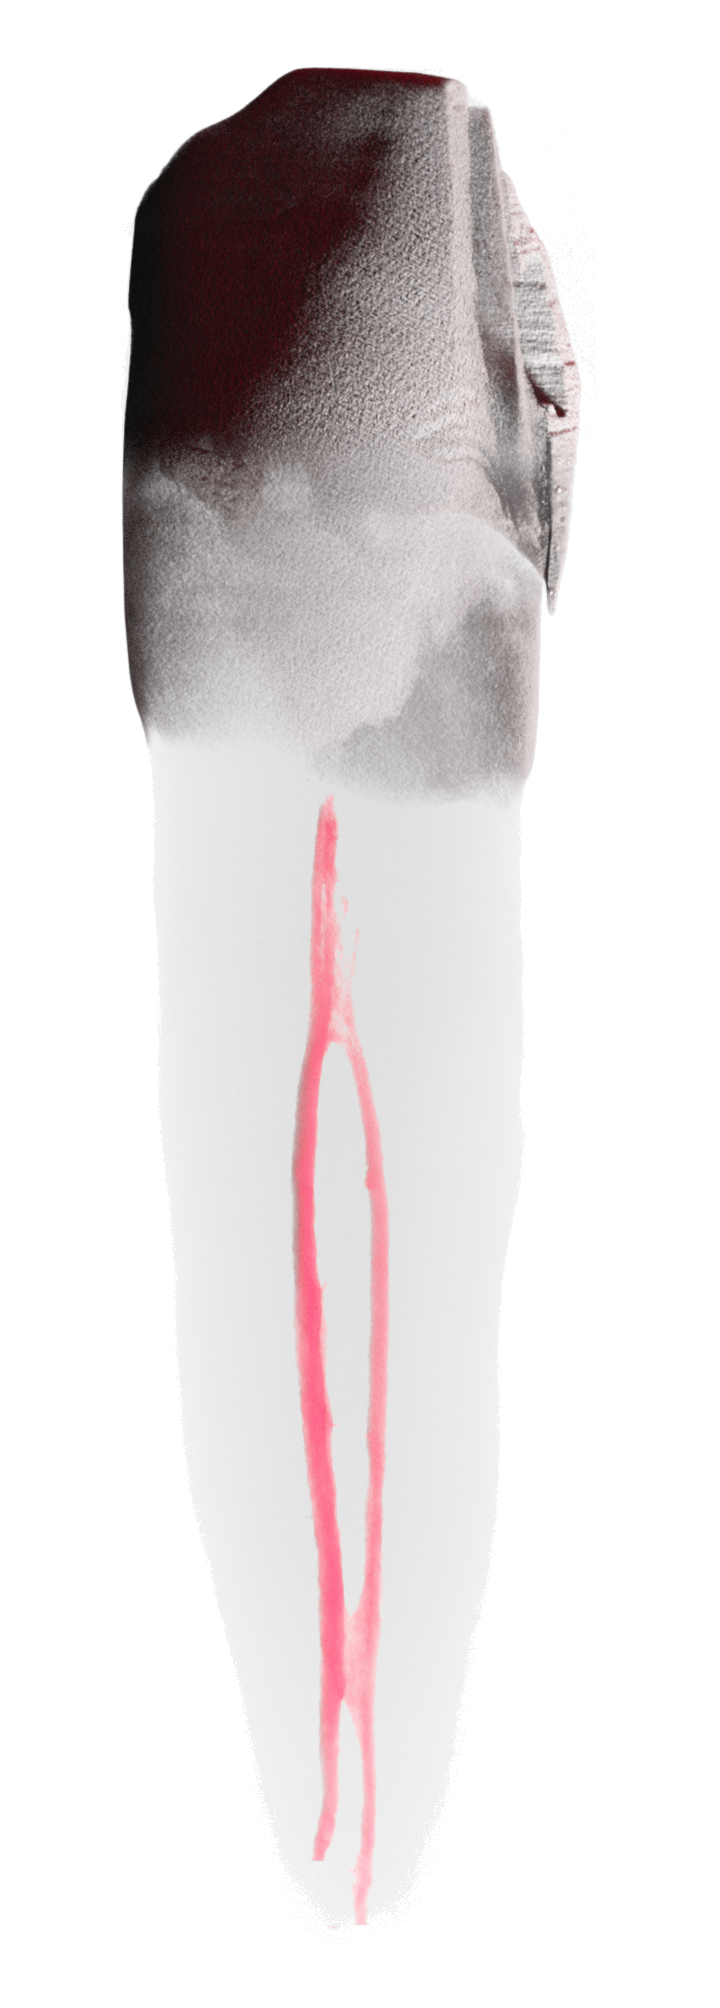
\includegraphics[height=\imheight]{./images/rcs/Tooth0452}%	
		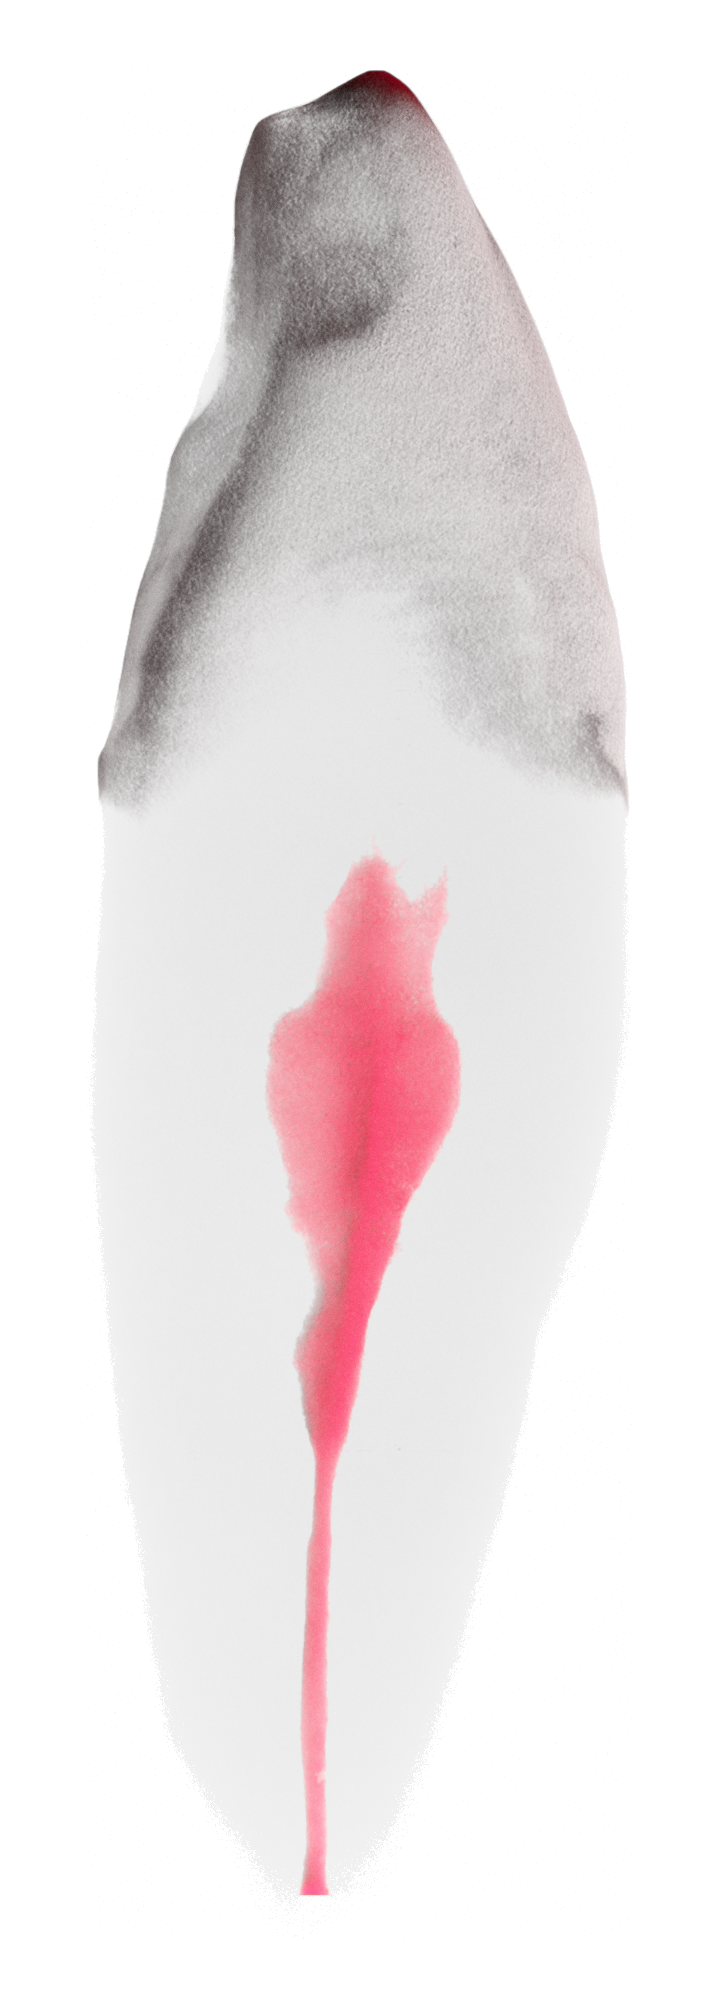
\includegraphics[height=\imheight]{./images/rcs/Tooth0278}%
		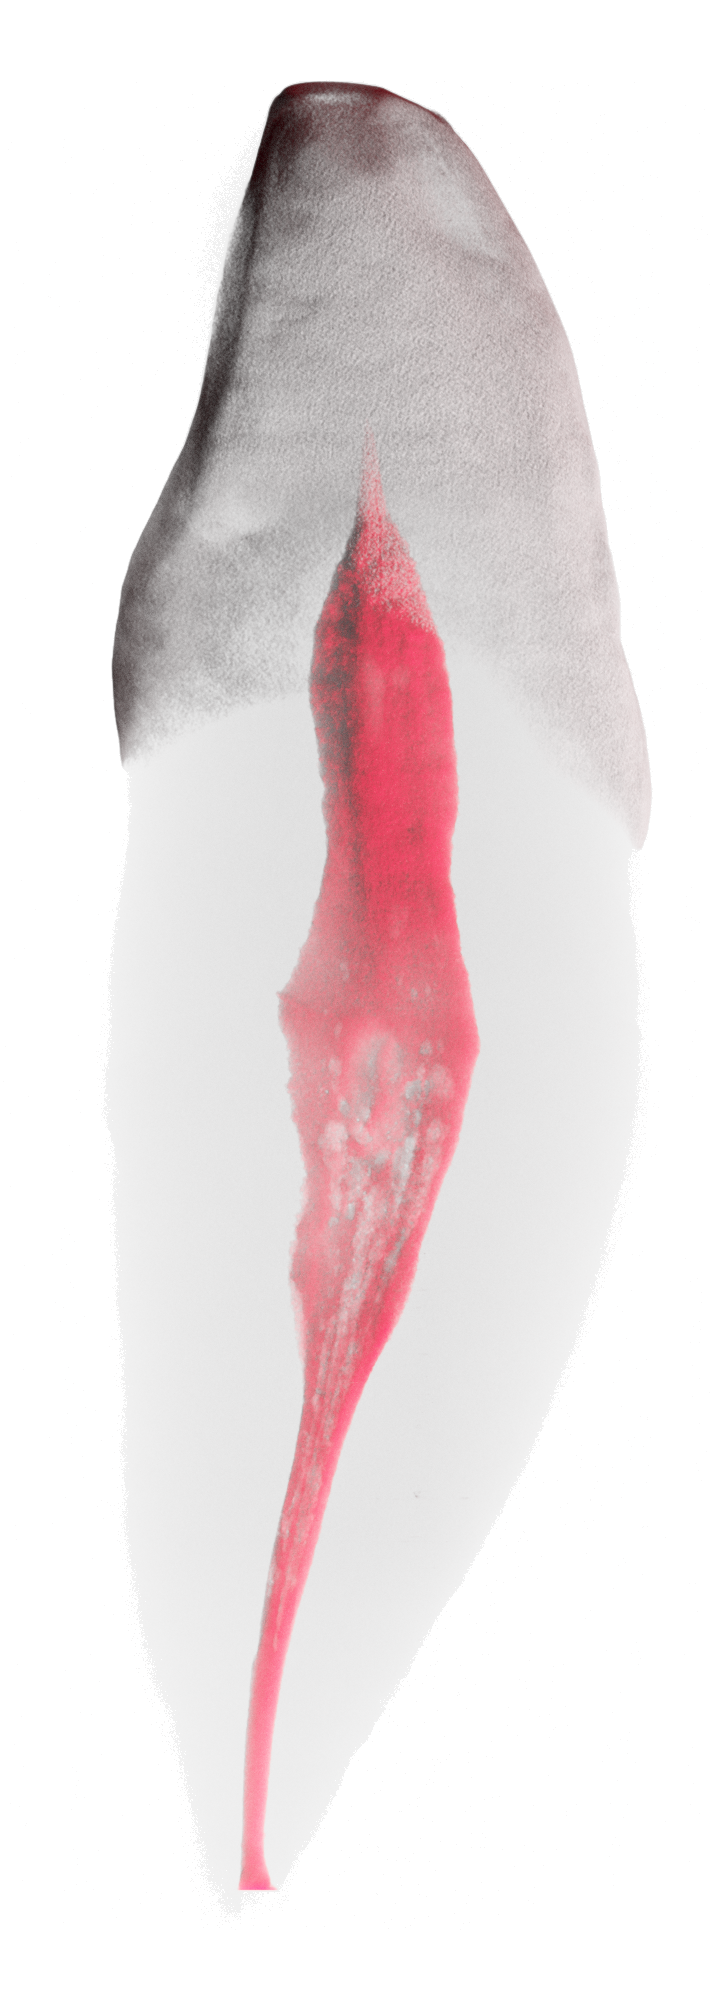
\includegraphics[height=\imheight]{./images/rcs/Tooth0353}%
		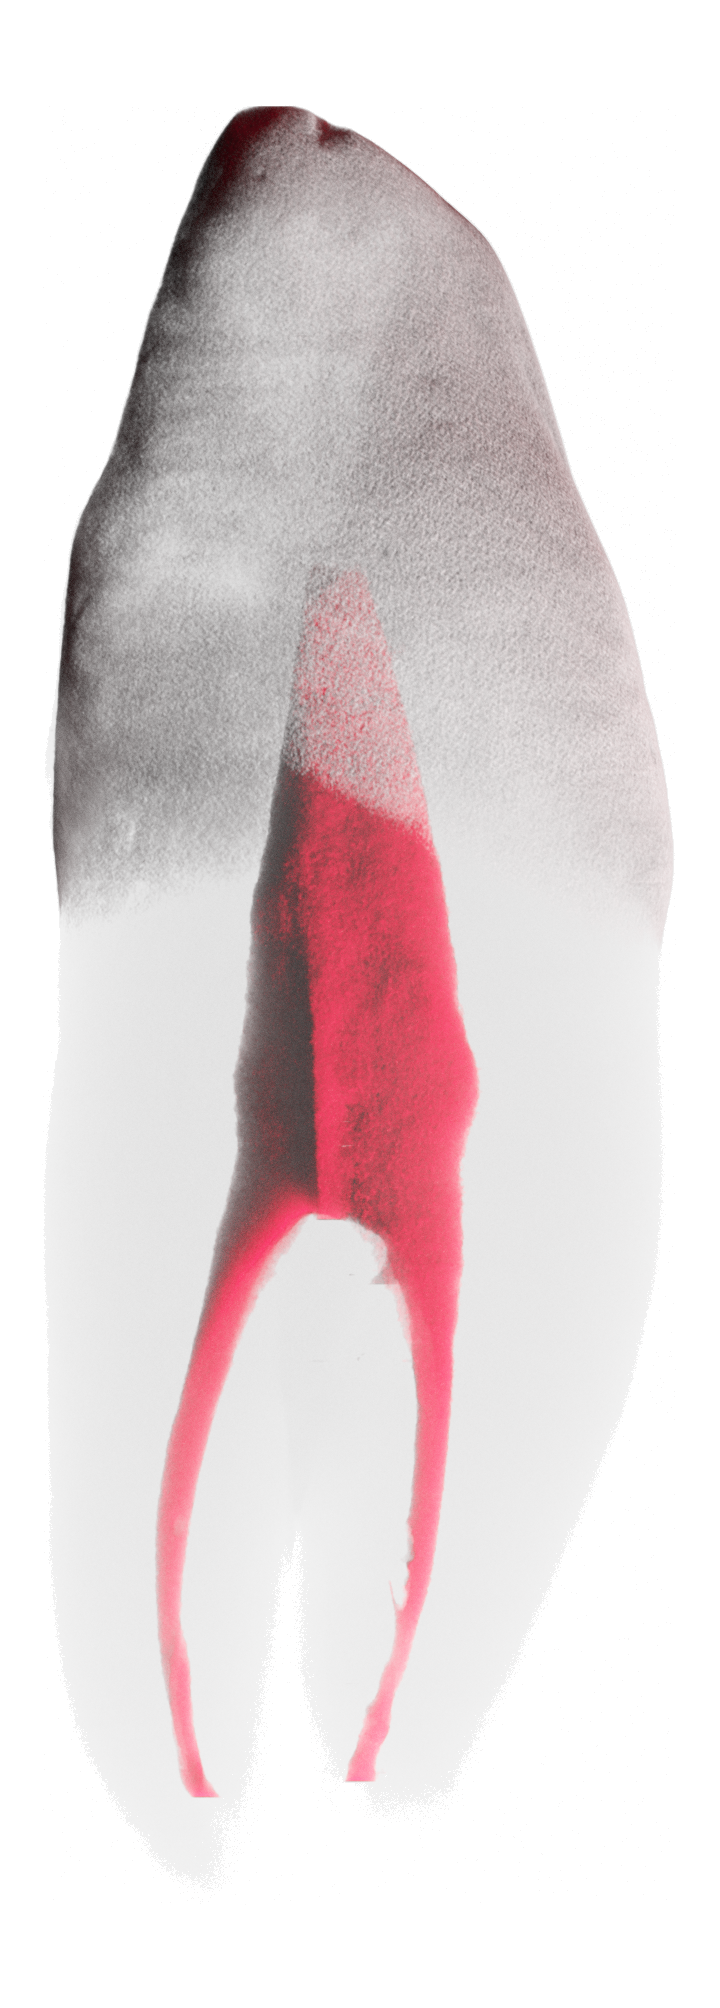
\includegraphics[height=\imheight]{./images/rcs/Tooth0419}%
		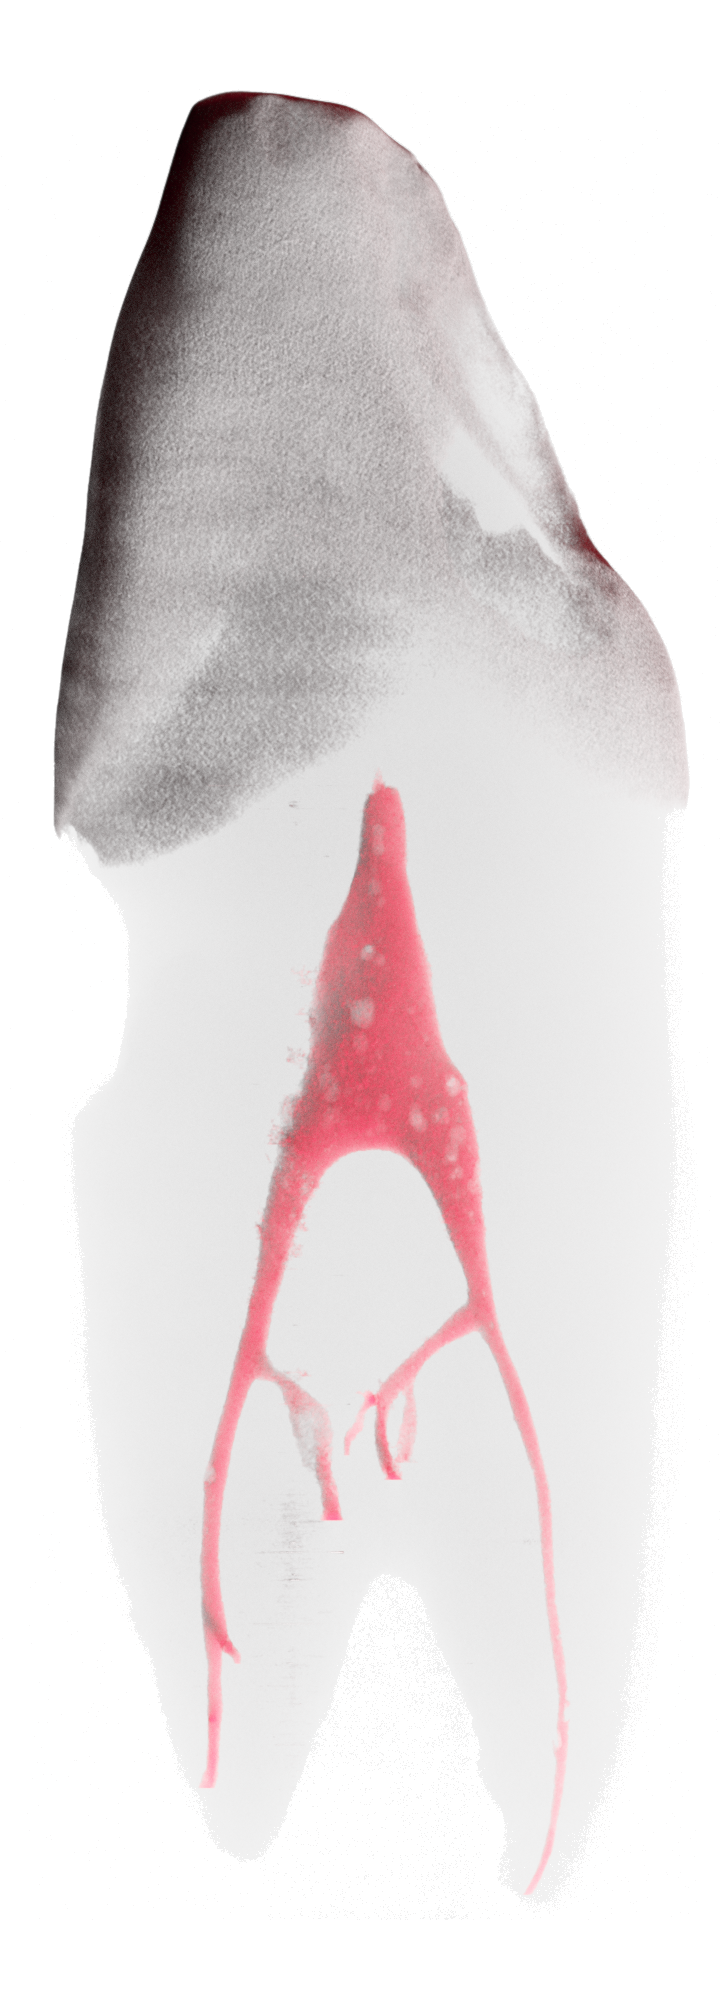
\includegraphics[height=\imheight]{./images/rcs/Tooth0642}%
		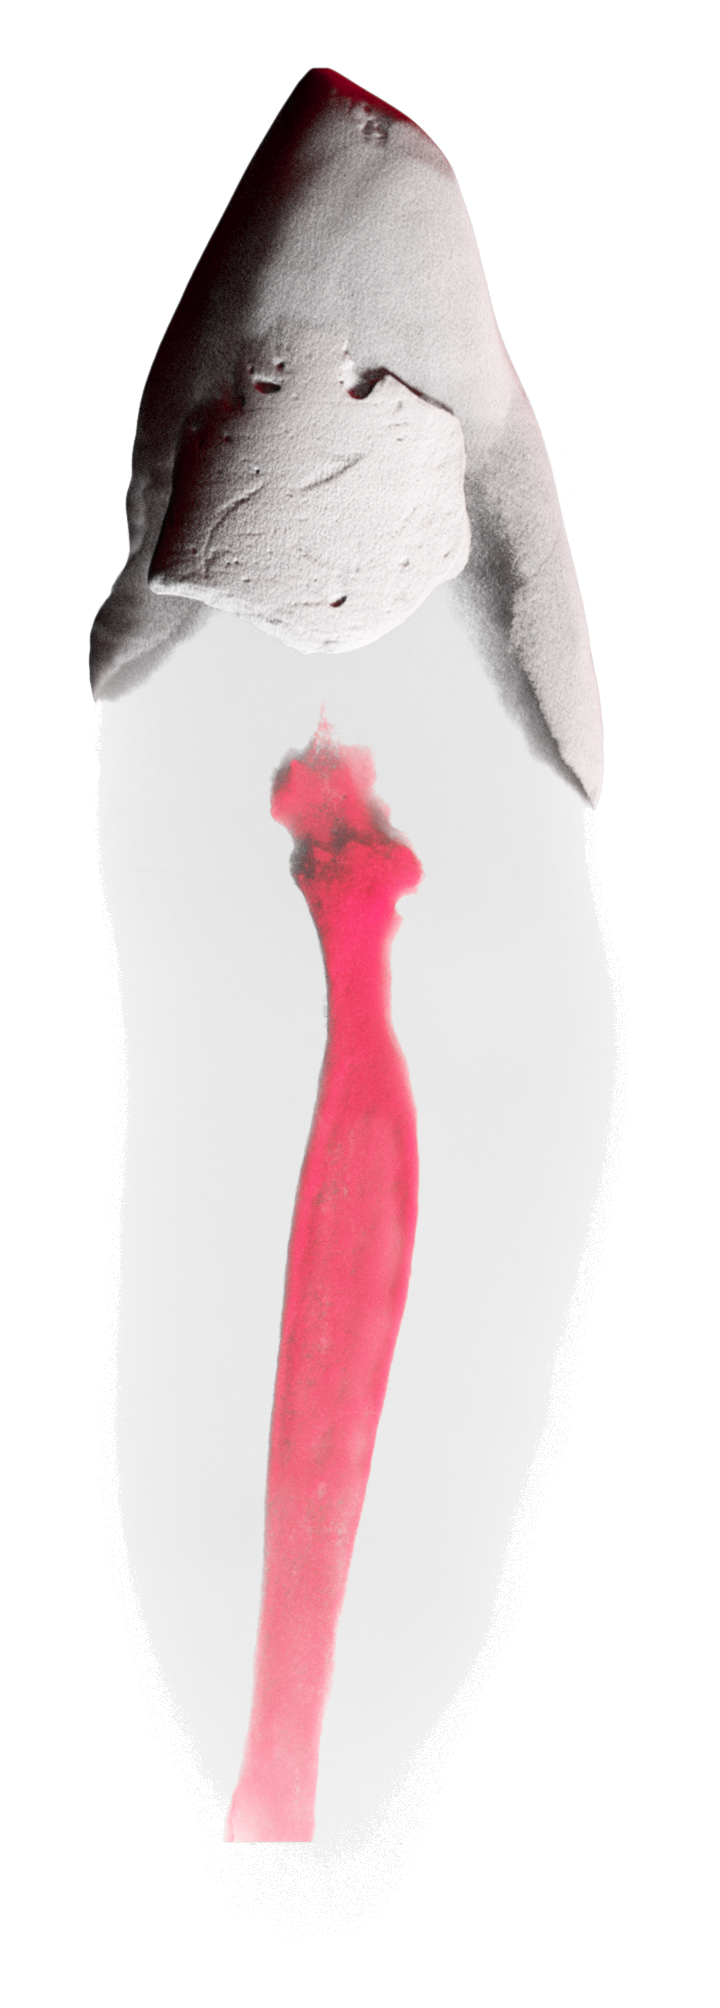
\includegraphics[height=\imheight]{./images/rcs/Tooth0752}%
		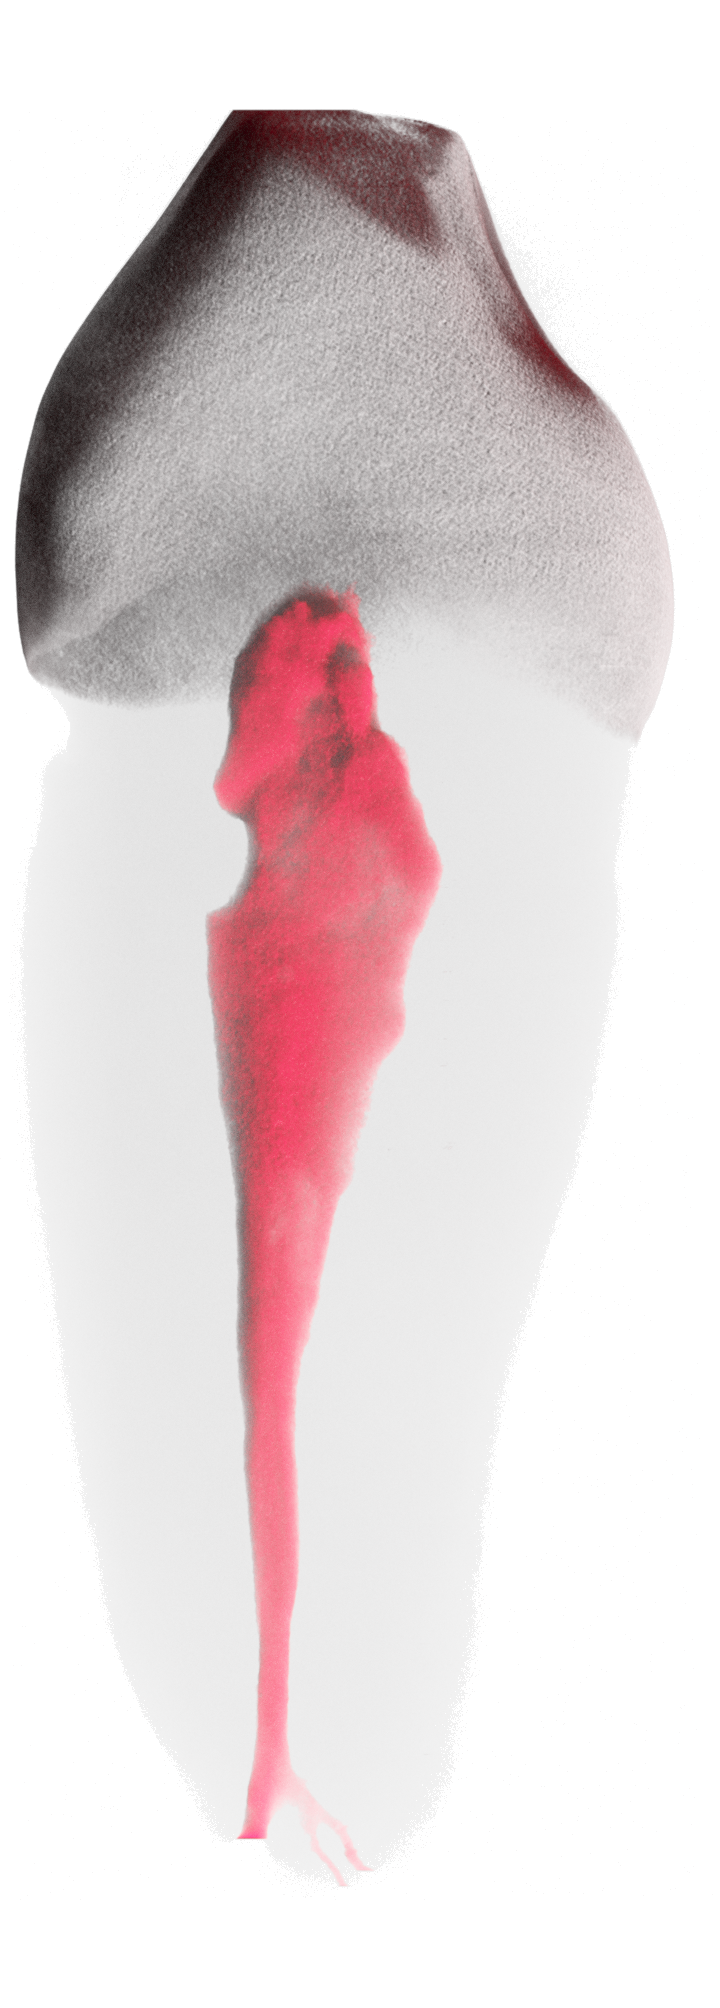
\includegraphics[height=\imheight]{./images/rcs/Tooth0931}%
\end{frame}

\begin{frame}
	\frametitle{Analysis of the physiological foramen geometry}
	\centering
	\only<1>{%
		\includegraphics[height=\imheight]{./images/foramen}%
		\sourcecite{Wolf2017}{Fig.~1}%
		}%
	\only<2>{%
		\animategraphics[palindrome,autoplay,height=\imheight]{24}{./movies/tooth045/edt-axial/Tooth045_EDT_Axial_}{100}{199}%
		}%
	\only<3>{%
		\animategraphics[palindrome,autoplay,height=\imheight]{24}{./movies/tooth045/edt-coronal/Tooth045_EDT_Coronal_}{123}{213}%
		}%
\end{frame}

\begin{frame}
	\frametitle{Outcome of foramen geometry analysis}
	\centering
	\begin{table}[]
		\begin{tabular}{cSSSSSSSS}
		\toprule
		& \multicolumn{2}{c}{1 Foramen} & \multicolumn{2}{c}{2 Foramina} & \multicolumn{2}{c}{3 Foramina} & \multicolumn{2}{c}{4 Foramina}\\
		& \#  & \% & \# & \% & \# & \% & \# & \%\\
		\midrule
		Oval		& 72 & 91.1 & 16 & 100.0 & 1 & 100.0 & 2 & 100.0\\
		Round		&  6 &  7.6 &    &       &   &       &   &\\
		Irregular	&  1 &  1.3 &    &       &   &       &   &\\
		\midrule
		N			& 79 &      & 16 &       & 1 &       & 2 &\\
		\bottomrule
		\end{tabular}
	\end{table}
\end{frame}

\begin{frame}
	\frametitle{Conclusion}
	\begin{itemize}
		\item Efficient use of time, \eg more teeth does not mean more (human) work
		\item Reproducible analysis with \emph{free and open-source} software, usable by \emph{anyone}
		\item Objective analysis, \eg no operator bias
	\end{itemize}
\end{frame}

\renewcommand{\imheight}{0.309\paperheight}%
\begin{frame}%
	\frametitle{Thanks!}%
	\begin{columns}%
		\begin{column}{0.5\linewidth}%
		\begin{itemize}%
			\item Topographic and clinical Anatomy%
			\begin{itemize}%
				\item Valentin Djonov, Ruslan Hlushchuk, Oleksiy-Zakhar Khoma and Jennifer Fazzari%
			\end{itemize}%
			\item zmk bern – Zahnmedizinische Kliniken%
			\begin{itemize}%
				\item Thomas G.\ Wolf, Andrea Anderegg and Michael Stiebritz%
			\end{itemize}%
			\item Swiss National Science Foundation%
			\item<2-> You, for listening to me%
			\item<3-> \href{https://twitter.com/ElaineLuther/status/1195708328854331392}{What can I clarify for you}?%
		\end{itemize}%
		\end{column}%
		\begin{column}{0.5\linewidth}%
			\centering%
			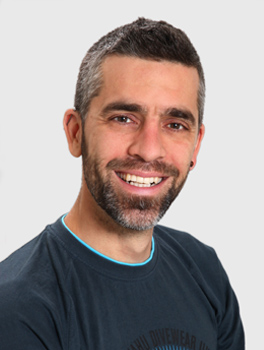
\includegraphics[height=\imheight]{./images/kopf_dh}%
			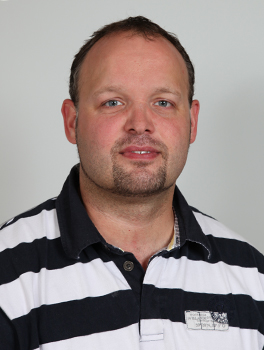
\includegraphics[height=\imheight]{./images/kopf_rh}\\%
			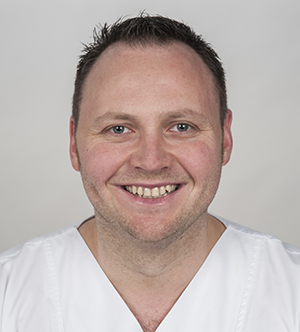
\includegraphics[height=\imheight]{./images/wolf_thomas_Web}%
			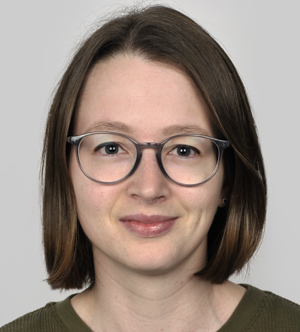
\includegraphics[height=\imheight]{./images/Anderegg_Andrea_web}%
		\end{column}%
	\end{columns}%
	\only<4>{%
		\begin{tikzpicture}[remember picture,overlay]%
			\node at (current page.center) [shift={(0,-25pt)}]{%
				\animategraphics[autoplay,loop,width=\paperwidth,every=\everyframe]{24}{./movies/tooth045/full-slices/image0}{000}{466}%
				};%
		\end{tikzpicture}%
	}%
\end{frame}

\begin{frame}[shrink] % `shrink' tries to autofit the content onto the slide, useful for very long lists of references
	\frametitle{References}
	% Make the references continuously smaller :)
	%\renewcommand*{\bibfont}{\small}
	%\renewcommand*{\bibfont}{\footnotesize}
	%\renewcommand*{\bibfont}{\scriptsize}
	\renewcommand*{\bibfont}{\tiny}
	\setbeamertemplate{bibliography item}{\insertbiblabel}
	\printbibliography
\end{frame}

\end{document}
